\begin{document}

The first inverter designed was the resistively loaded NMOS transitor. This designed features only one NMOS transistor in series with a resistor. The source is supplied some voltage and driven with a PWM source. The analysis of the NMOS circuit stems from two extreme cases: 1) the input V$_{gate}$ is 0V and the voltage at the drain, V$_{drain}$ = V$_{DD}$ and 2) input V$_{gate}$ = V$_{DD}$ and output V$_{drain}$=0V. Case 1) describes the state in which no current is flowing through the MOSFET and the it is operating in cut-off. Case 2) described the state in which the transistor is operating in the triode region. The current through the MOSFET is described by Equation \ref{eqn:mosfetcurrent}

\begin{equation}
I_{DS} = \mu_n C_{ox}\frac{W}{L}[(V_{GS}-V_t)V_{DS}-\frac{1}{2}V^{2}_{DS}],
\label{eqn:mosfetcurrent}
\end{equation}

where the drain current is found to be equal the hole mobility $\mu_n$, the capacitance between the oxide terminals, the ratio of the width to the length of the channel, and V$_t$ is the threshold voltage. 
\newline

The design for resistively loaded followed by solving for an arbitrary input. For the purpose of this lab we are interested in V$_{out}$=2.5 when V$_in$=2.5 \cite{b2}. From these assumptions, it follows that V$_{GS}$ $>$ V$_t$ so the MOSFET is on, but somewhere in the triode to saturation range. It is known from V$_{DS}$ $>$ V$_{GS}$ that the MOSFET is in fact in saturation. Equation \ref{eqn:mosfetcurrent} simplifies to Equation \ref{eqn:mosfetsimp}

\begin{equation}
I_{DS} = \mu_n C_{ox}\frac{W}{L}[(V_{GS}-V_t)^2],
\label{eqn:mosfetsimp}
\end{equation}

where the drain current now only depends on the gate voltage and the threshold voltage. For the CD4007, the k' parameter, seen in Equation \ref{eqn:kprime}

\begin{equation}
k' = \mu_n C_{ox}\frac{W}{L},
\label{eqn:kprime}
\end{equation}

where k' is equal to approximately 500$\frac{\mu A}{V^2}$.
From this current the load resistance can be found by application of Ohm's Law, which results in 4.4k$\Omega$. The circuit was simulated using NGspice integrated with Matlab. The simulated circuit is shown in Figure \ref{fig:simcircuit}.


\begin{figure}[H]
    \centering
    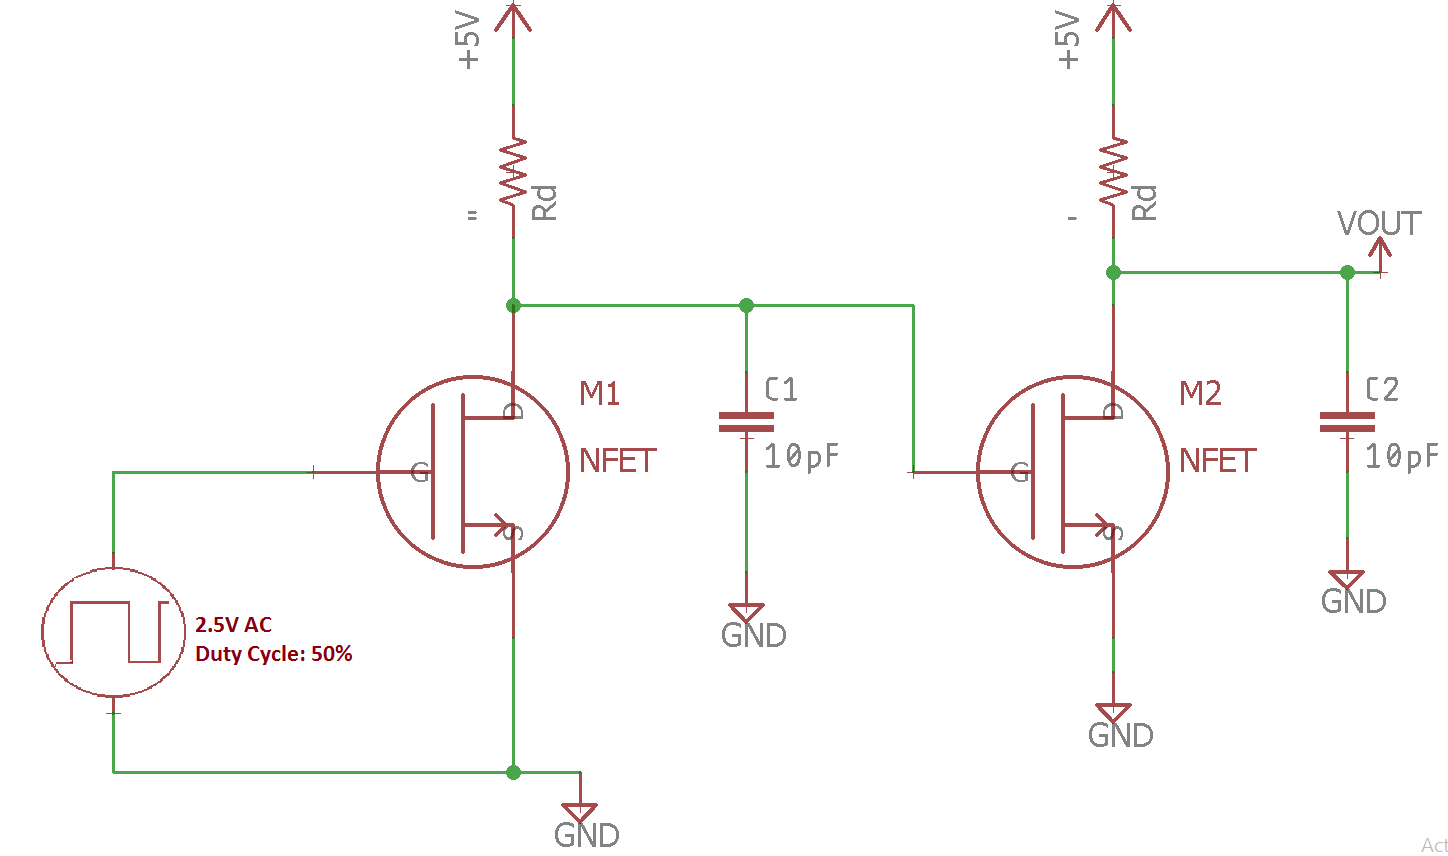
\includegraphics[scale = .25]{CircuitDevelopment/NMOS/DuelNMOS.png}
    \caption{Simulated NMOS inverter}
    \label{fig:simcircuit}
\end{figure}

The parasitic capacitance of the breadboard was approximated by the inclusion of the 10pF capacitors at the outputs of the inverters. Figure \ref{fig:NMOSvsR} demonstrates the output voltage as a function of the load resistance. The output voltage was measured while performing a sweep of resistor values.

\begin{figure}[H]
    \centering
    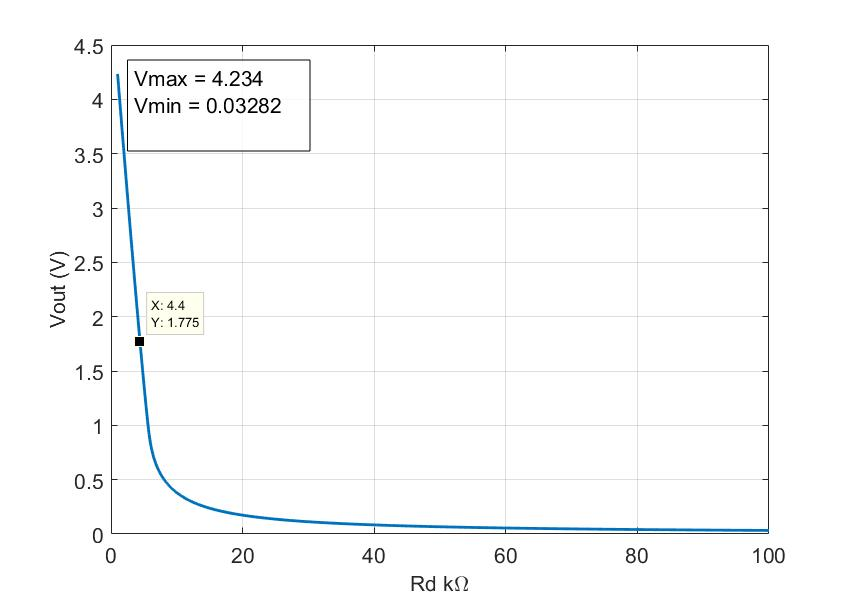
\includegraphics[scale = .30]{CircuitDevelopment/NMOS/voutvsrd_nmos_inverter.jpg}
    \caption{Simulated NMOS Vout vs R}
    \label{fig:NMOSvsR}
\end{figure}

The position of the calculated resistance in Figure \ref{fig:NMOSvsR} demonstrates the simulated output voltage at a 4.4k$\Omega$ value. Notably, the upper threshold of effective resistor values is around 9k$\Omega$. The VTC of the NMOS inverter is shown in Figure \ref{fig:VTCNMOS} for three resistor values.

\begin{figure}[H]
    \centering
    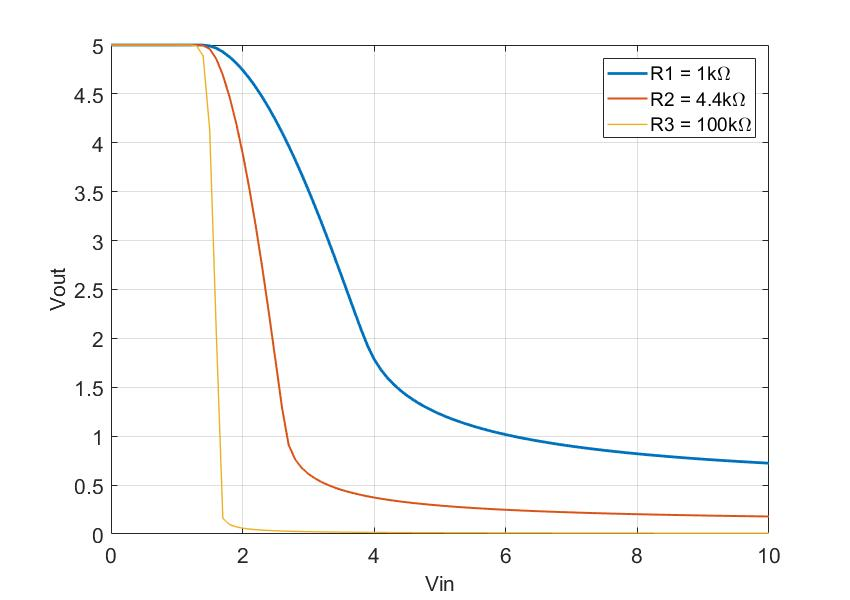
\includegraphics[scale = .30]{CircuitDevelopment/NMOS/VTC_single_NMOS.jpg}
    \caption{Simulated VTC of single NMOS inverter}
    \label{fig:VTCNMOS}
\end{figure}

 The 100k$\Omega$ resistor features the most abrupt transition between logic states. The voltage at which it transitions, however, is below the supplied V$_{in}$ of 2.5V, meaning this gate would subsequently change states at incorrect voltages. The 4.4k$\Omega$ resistor produces a transition at the voltage 2.5V, as calculated. 
\newline

The transient analysis of the NMOS inverter was performed in NGSpice in conjunction with MATLAB. The time-domain graph of the inverter with a resistance of 1k$\Omega$ is shown in Figure \ref{fig:1ktran}.

\begin{figure}[H]
    \centering
    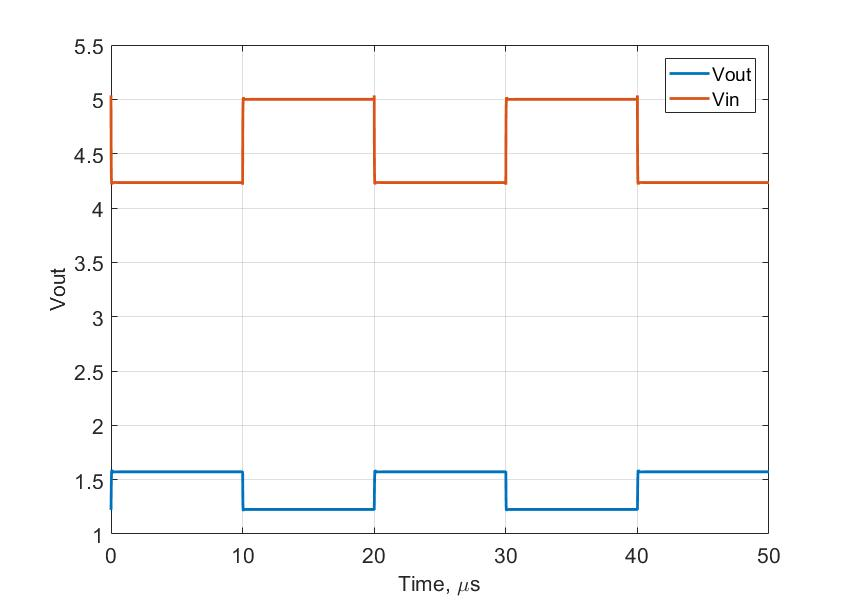
\includegraphics[scale = .30]{CircuitDevelopment/NMOS/tran_1k_nmos.jpg}
    \caption{Simulated transient with 1k resistor}
    \label{fig:1ktran}
\end{figure}

The output voltage is far below that of the input voltage in \ref{fig:1ktran}. The output waveform had a rise time of 129ns and a fall time of 122ns. The output waveform can then be contrasted with the output voltage calculated using a 4.4k$\Omega$ resistor seen in Figure \ref{fig:4ktran}.

\begin{figure}[H]
    \centering
    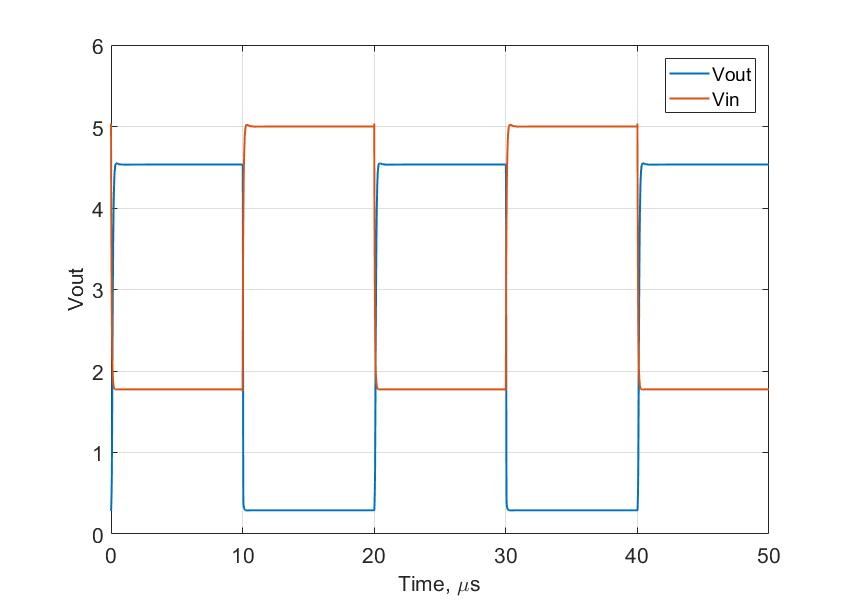
\includegraphics[scale = .30]{CircuitDevelopment/NMOS/tran_4k_nmos.jpg}
    \caption{Simulated transient with 4.4k resistor}
    \label{fig:4ktran}
\end{figure}

The output voltage, as seen in Figure \ref{fig:4ktran}, now outputs a voltage that is very nearly the supply voltage. The rise time was found to be 1.15 $\mu$s and the fall time was 133ns. The time-domain voltages for the 100k$\Omega$ resistor was also found, as shown in Figure \ref{fig:100ktran}. 

\begin{figure}[H]
    \centering
    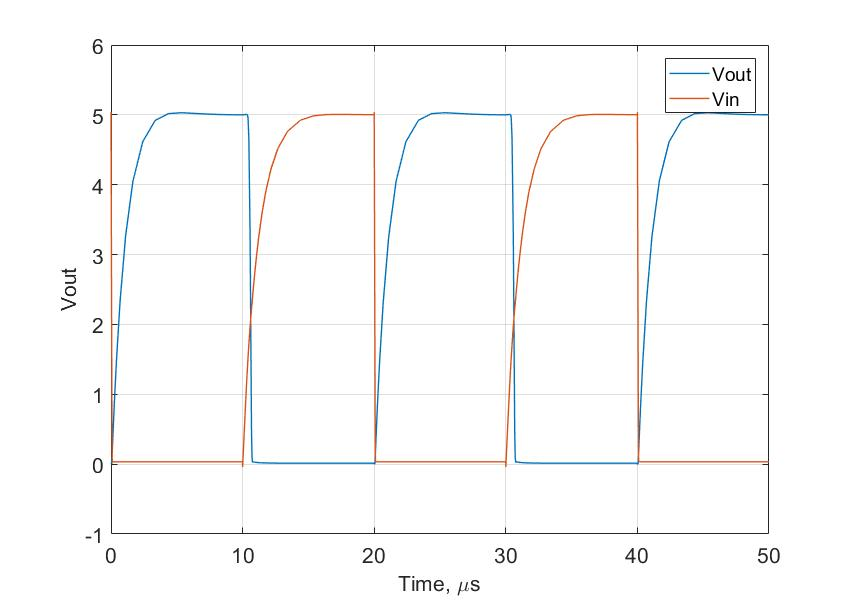
\includegraphics[scale = .30]{CircuitDevelopment/NMOS/tran_100knmos.jpg}
    \caption{Simulated transient with 100k resistor}
    \label{fig:100ktran}
\end{figure}

The introduction of the 100k$\Omega$ resistor dramatically increased the rise time of the output waveform. The rise time was found to be 12.1$\mu$s with a fall time of 1.19$\mu$s. The larger resistance increased the time constant of the equivalent RC circuit from the resistor and parasitic capacitance. The supply voltage was also increased in order to determine the effect on the inverter. Figure \ref{fig:10vtran} shows the output voltage with a 10V supply and the 4.4k$\Omega$ resistor.

\begin{figure}[H]
    \centering
    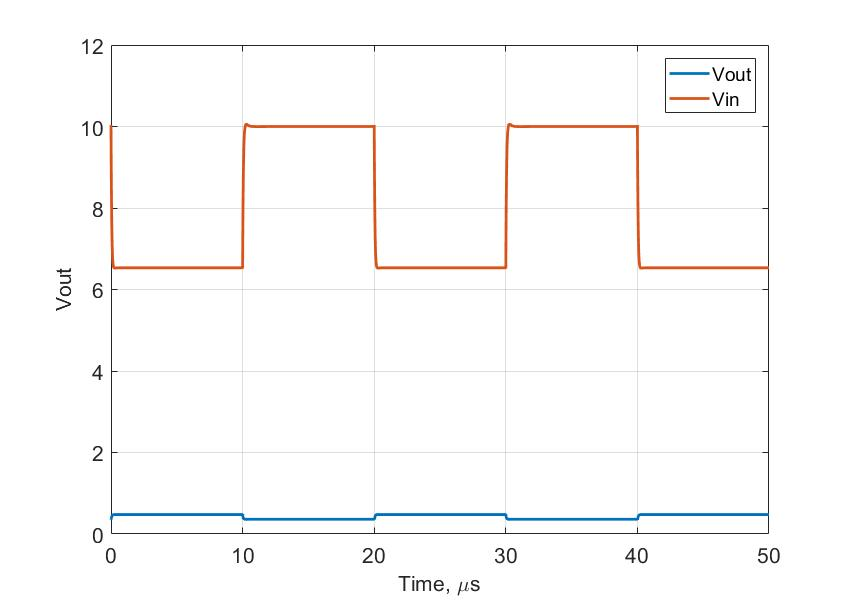
\includegraphics[scale = .30]{CircuitDevelopment/NMOS/tran_4k_vdd_10.jpg}
    \caption{Simulated transient with 4.4k resistor and 10V supply}
    \label{fig:10vtran}
\end{figure}

The output voltage decreases with the supply voltage, which agrees with Equation \ref{eqn:mosfetsimp}. The rise time was then found to be 1.11$\mu$s with a fall time of 185ns. The disparity between the supply voltage and the output voltage is seen when the supply is increased to 15V, as show in Figure \ref{fig:15vtran}.


\begin{figure}[H]
    \centering
    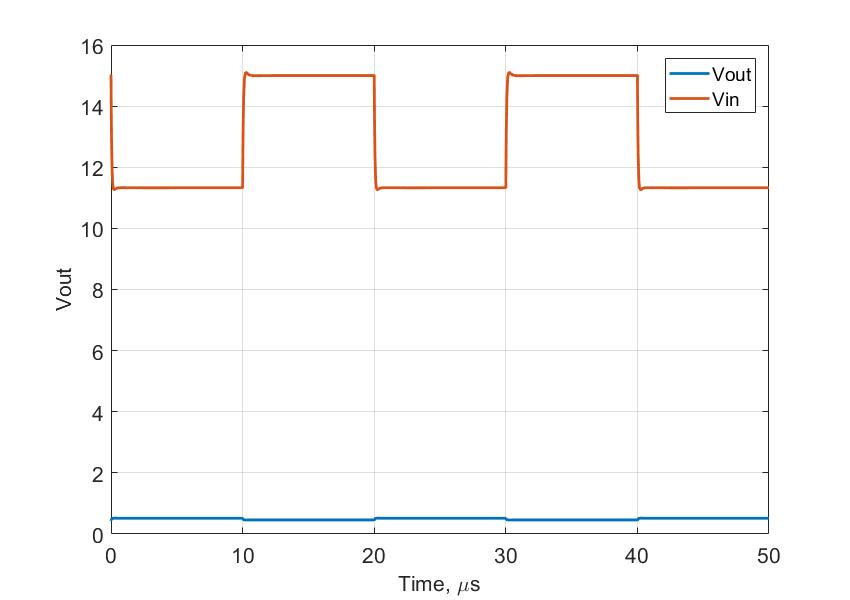
\includegraphics[scale = .30]{CircuitDevelopment/NMOS/tran_4k_vdd_15.jpg}
    \caption{Simulated transient with 4.4k resistor and 15V supply}
    \label{fig:15vtran}
\end{figure}

The rise and fall times were found to be 199ns and 195ns respectively. The supply voltage did not play a significant role in rise or fall times, but did dramatically alter the output voltage. Table \ref{tab:NMOS} shows the simulated results for the NMOS inverter.



\begin{table}[H]
\centering
\caption{NMOS simulated results}
\label{tab:NMOS}
\begin{tabular}{|l|l|}
\hline
Values    & Results      \\ \hline
R         & 4.4k$\Omega$ \\ \hline
Min Power & 69.5pW       \\ \hline
Max Power & 31.2mW       \\ \hline
V$_{max}$ & 4.23V        \\ \hline
V$_{min}$ & 32.8mV       \\ \hline
Rise Time & 129ns        \\ \hline
Fall Time & 122ns        \\ \hline
\end{tabular}
\end{table}

The simulated results were in line with the theoretical values, the inverters operated as expected.










\end{document}